\documentclass[11pt,dvipsnames,usenames,aspectratio=169]{beamer}  % Add handout to options to disable overlays

% For more themes, color themes and font themes, see:
% http://deic.uab.es/~iblanes/beamer_gallery/index_by_theme.html
%
\mode<presentation>
{%
  \usetheme{CambridgeUS}    % or try default, Darmstadt, Warsaw, ...
  \usecolortheme{whale}     % or try albatross, beaver, crane, ...
  \usefonttheme{serif}          % or try default, structurebold, ...
  % \usefonttheme[onlymath]{serif}
  % \setbeamertemplate{navigation symbols}{}
  % \setbeamercovered{transparent}

  \setbeamercolor{title}{fg=white}
  \setbeamerfont{title}{series=\bfseries}
  \setbeamercolor{frametitle}{fg=black}
  \setbeamerfont{frametitle}{series=\bfseries}

  \setbeamercolor{section in head/foot}{fg=white}
  \setbeamerfont{section in head/foot}{series=\bfseries}
  \setbeamercolor{subsection in head/foot}{fg=white}
  \setbeamerfont{subsection in head/foot}{series=\bfseries}
  \setbeamercolor{author in head/foot}{fg=white}
  \setbeamerfont{author in head/foot}{series=\bfseries}
  \setbeamercolor{title in head/foot}{fg=white}
  \setbeamerfont{title in head/foot}{series=\bfseries}

  \setbeamercolor{block title}{use=structure,fg=white,bg=title in head/foot.bg}
  \setbeamerfont{block title}{series=\bfseries}
  \setbeamercolor{block body}{use=structure,fg=black,bg=black!1!white}
}

% Support graying out frame elements
\newcommand{\FrameOpague}{\setbeamercovered{again covered={\opaqueness<1->{40}}}}
% Transition slide
\newcommand{\transitionFrame}[1]{%
{%
  \begin{frame}[plain,noframenumbering]{}{} % the plain option removes the sidebar and header from the title page
    \setbeamertemplate{final page}[text]{\Large \textbf{#1}}
    \usebeamertemplate{final page}
  \end{frame}}
}

% Imported via UltiSnips
\usepackage{graphicx} % Loading the package
\graphicspath{{img/}} % Setting the default folder containing the graphics

\usepackage[numbers]{natbib}
\usepackage{appendixnumberbeamer}

% Here's where the presentation starts, with the info for the title slide
\title[Principles Explainable ML]{Principles and Practice of Explainable Machine Learning}
\author[Belle \& Papantonis]{%
  {Vaishak Belle}\inst{1}\inst{2}
  \and
  {Ioannis Papantonis}\inst{1}
}

\institute[U.\ Edinburgh]{%
  \textsuperscript{1}\textbf{University of Edinburgh}
  \and
  \textsuperscript{2}\textbf{Alan Turing Institute}
}
\date{October~8, 2020}

% Imported via UltiSnips
\newcommand{\etal}{~et~al.}

% Used for including standalone docs
\usepackage{standalone}

% Imported via UltiSnips
% Unbreakable dash:
%  Words hyphened with these dashes can also be broken at other positions than the dash
%    \-/ hyphen
%    \-- en-dash
%    \--- em-dash
%    extdash unbreakable dashes
%
%  No line breaks possible at the hyphen
%    \=/ hyphen
%    \== en-dash
%    \=== em-dash
\usepackage[shortcuts]{extdash}

% Imported via UltiSnips
% \usepackage{xcolor}
\newcommand{\colortext}[2]{{\color{#1} #2}}
\newcommand{\red}[1]{\colortext{red}{#1}}
\newcommand{\blue}[1]{\colortext{blue}{#1}}
\newcommand{\green}[1]{\colortext{ForestGreen}{#1}}

% Imported via UltiSnips
\usepackage{amsmath}
\DeclareMathOperator*{\argmax}{arg\,max}
\DeclareMathOperator*{\argmin}{arg\,min}
\usepackage{amsfonts}  % Used for \mathbb and \mathcal
\usepackage{amssymb}

% Imported via UltiSnips
\usepackage{mathtools} % for "\DeclarePairedDelimiter" macro
% \swapifbranches changes unstarred paired delimiters to starred and
% vice versa.  This means by default, paired delimiters have the star.
\usepackage{etoolbox}
\newcommand\swapifbranches[3]{#1{#3}{#2}}
\makeatletter
\MHInternalSyntaxOn
\patchcmd{\DeclarePairedDelimiter}{\@ifstar}{\swapifbranches\@ifstar}{}{}
\MHInternalSyntaxOff
\makeatother
% Place after swap to ensure swap star
\DeclarePairedDelimiter{\sbrack}{\lbrack}{\rbrack}
\DeclarePairedDelimiter{\floor}{\lfloor}{\rfloor}
\DeclarePairedDelimiter{\ceil}{\lceil}{\rceil}
\DeclarePairedDelimiter{\abs}{\lvert}{\rvert}
\DeclarePairedDelimiter{\round}{\lfloor}{\rceil}
\DeclarePairedDelimiter{\norm}{\lVert}{\rVert}
\usepackage{bm}
\DeclarePairedDelimiterX\set[1]\lbrace\rbrace{#1}
\DeclarePairedDelimiterX\setbuild[2]\lbrace\rbrace{#1 \bm: #2}
\newcommand{\setint}[1]{{\sbrack{#1}}}
\newcommand{\func}[3]{{#1:#2\rightarrow#3}}
% \newcommand{\defeq}{\stackrel{\mathclap{\mbox{\tiny def}}}{=}}
\newcommand{\defeq}{\coloneqq}
\newcommand{\fedeq}{\eqqcolon}
\newcommand{\expect}[1]{\mathbb{E}\sbrack{#1}}
% Expectation with the subscript defining the distribution
\newcommand{\expectS}[2]{\mathbb{E}_{#1}\sbrack{#2}}

% Allow numbering in align*
\newcommand{\numberthis}{\addtocounter{equation}{1}\tag{\theequation}}

\newcommand{\ints}{\mathbb{Z}}
\newcommand{\intsNN}{\mathbb{Z}_{+}}
\newcommand{\nats}{\mathbb{N}}
\newcommand{\real}{\mathbb{R}}
\newcommand{\realnn}{\real_{{\geq}0}}  % Set of non-negative real numbers

\newcommand{\iidsim}{\stackrel{\mathclap{\mbox{\tiny \textnormal{i.i.d.}}}}{\sim}}

\newcommand{\normaldist}[2]{{\mathcal{N}\mathopen{}\left(#1,#2\right)\mathclose{}}}

% Imported via UltiSnips
\usepackage{array}  % Provides a way add a \centering command to a p-column
\usepackage{arydshln}  % Introduces hdashline & cdashline
\usepackage{bigdelim}
\usepackage{booktabs}
\usepackage{multirow}
\usepackage{makecell}  % Needed for multirowcell

% % Imported via UltiSnips
\usepackage{amsthm}
% \newtheorem{theorem}{Theorem}
% \newtheorem{corollary}{Corollary}[theorem]  % Corollary number derives from theorem
% \newtheorem{lemma}[theorem]{Lemma}  % Lemma and theorem share same counter
% \newtheorem{claim}[theorem]{Claim}  % Same numbering as lemma and theorem
% \newtheorem*{remark}{Remark}
% \newtheorem*{note}{Note}
% \newtheoremstyle{definition}  % <name>
% {3pt}   % <Space above>
% {3pt}   % <Space below>
% % {\itshape}     % <Body font>
% {\normalfont}   % <Body font>
% {}      % <Indent amount>
% {\bfseries} % <Theorem head font>
% {:}     % <Punctuation after theorem head>
% {.5em}  % <Space after theorem head>
% {}      % <Theorem head spec (can be left empty, meaning `normal')>
% \theoremstyle{definition}
% \newtheorem{definition}{Def.}[section]

% Imported via UltiSnips
\usepackage{tikz}
\usetikzlibrary{arrows,decorations.markings,shadows,positioning,calc,backgrounds,shapes}

\usepackage{pgfplots}
\pgfplotsset{compat=1.13}
\usepackage{pgfplotstable}
% \usepackage{subcaption}  % Cannot be used with subfigure

% Handle empty parameters
\usepackage{xifthen}
\newcommand{\ifempty}[3]{%
  \ifthenelse{\isempty{#1}}{#2}{#3}%
}

\newcommand{\dec}{f}
\newcommand{\domainX}{X}
\newcommand{\domainY}{Y}

\newcommand{\X}{x}

\newcommand{\dist}{\mathcal{D}}

\newcommand{\Rule}{A}
\newcommand{\setRule}{\mathcal{A}}
\newcommand{\predicate}{a}

\newcommand{\Prec}[1]{{\text{prec}(#1)}}
\newcommand{\minPrec}{\tau}

\newcommand{\cov}[1]{{\text{cov}(#1)}}
\newcommand{\minCov}{c}

\newcommand{\beamWidth}{B}


% Enable (uncolored) cross-reference hyperlinks
% Should always be last package loaded.
% See: https://tex.stackexchange.com/questions/103123/links-do-not-lead-to-right-pages
\usepackage{hyperref}

\begin{document}

\begin{frame}
  \titlepage
\end{frame}

\section{Case Study}
\begin{frame}{Let's Start with a Case Study\ldots}
  \noindent
  Before examining the problem from a technical perspective, let's think through a \textit{real-world} scenario
  \begin{itemize}
    \item Help us identify salient ideas
    \item Allow us to construct a working vocabulary
  \end{itemize}

  \vspace{18pt}
  \onslide<2->{
    \noindent
    \textbf{Note}: A case study appears at the end of paper, but I think the following will yield a more fruitful discussion.
  }
\end{frame}

\begin{frame}{Fair Criminal Sentencing}
  \begin{itemize}[<+->]
    \setlength{\itemsep}{22pt}
    \onslide<+->{\item I get this is a bit heavy topic\ldots}

    \onslide<+->{\item \textbf{Sentence}: Punishment (e.g.,~fine, probation, imprisonment, restituion) assigned in relation to a specific criminal act.}

    \onslide<+->{\item \green{\textbf{Accurate}}/appropriate sentencing is \textbf{critical} for a healthy justice system.}

    \onslide<+->{%
      \item \textbf{Key Attributes of an Appropriate Sentencing Apparatus}
      \begin{itemize}
        \setlength{\itemsep}{3pt}
        \item \textit{Consistent}: Similar crimes/circumstances should yield similar punishments.
        \item \textit{Understandable}: Clarity \textit{why} the selected sentence is appropriate
        \item \textit{Transparent}: Knowledge of \textit{how} the sentence was selected sentence
        \item \textit{Sufficient}: Ensures justice for the victims and keeps the public safe
      \end{itemize}
    }
  \end{itemize}
\end{frame}

\begin{frame}{Problem with Sentencing Today}
  \onslide<+->{\textbf{\blue{Major Problem}}: Human juries/judges badly affected by bias\ldots}

  \onslide<+->{%
    \begin{itemize}
      \setlength{\itemsep}{22pt}
      \item \textbf{Racial Bias}: An African-American defendant is 5.9x as likely to be imprisoned as a white defendant. Hispanics are 3.1x as likely.~\citep{SentencingProject}

      \item \textbf{Gender Bias}: Men receive 63\% longer sentences on average than women do. Women are twice as likely to avoid incarceration if convicted.~\citep{Starr:2014}

      \item \textbf{Wealth Effects}: Poor defendants more likely to plead guilty since they cannot afford bail and lack a safety net to afford remaining in prison until trial
    \end{itemize}
  }
\end{frame}

\subsection{AI \& the Justice System}
\begin{frame}{Here's an Idea\ldots}
  \onslide<+->{Take the \textit{humans} out of sentencing
    \begin{itemize}
      \item Make it entirely ``data driven''
    \end{itemize}
  }

  \vspace{22pt}
  \onslide<+->{%
    Use machine learning to estimate the \green{recidivism rate}. \textbf{Three types of recidivism}:
    \begin{itemize}
      \item \textit{Pretrial recidivism}
      \item \textit{General recidivism}
      \item \textit{Pretrial recidivism}
    \end{itemize}
  }

  \vspace{22pt}
  \onslide<+->{\blue{\textbf{COMPAS}}: \underline{C}orrectional \underline{O}ffender \underline{M}anagement \underline{P}rofiling for \underline{A}lternative \underline{S}anctions
    \begin{itemize}
      \item Released: 2009
      \item \green{\textbf{Proprietary}} (Developed by private company Northpointe)
    \end{itemize}
  }
\end{frame}

\begin{frame}{You May See Where This is Going\ldots}
  \begin{center}
    \onslide<2->{
      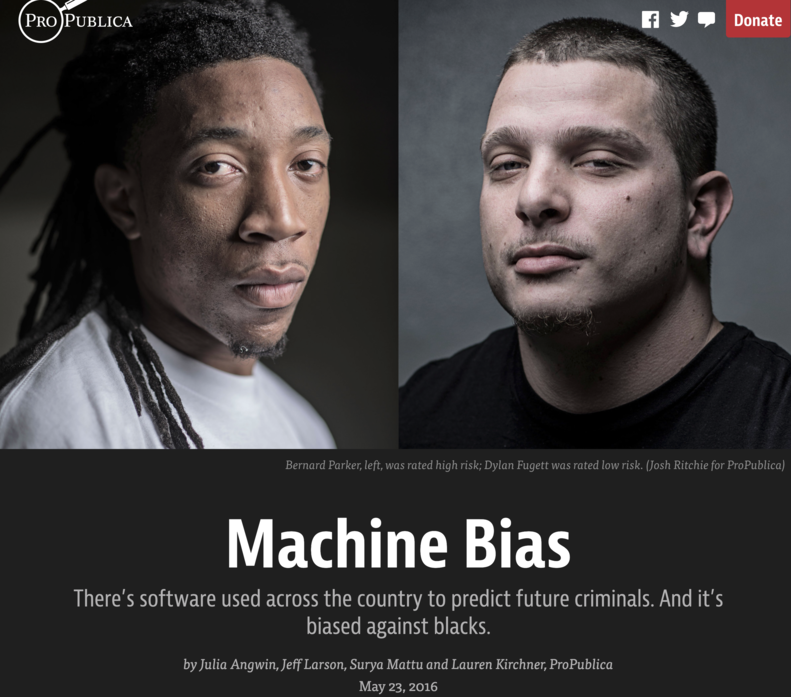
\includegraphics[scale=0.55]{propublica_compas_small.png}
    }
  \end{center}
\end{frame}

\begin{frame}{Some of the Highlights (or Lowlights)\ldots}
  \noindent
  \onslide<+->{\textbf{Source}:~\citet{Angwin:2016} (7~years after COMPAS' initial release)}

  \begin{itemize}[<+->]
    \setlength{\itemsep}{12pt}
    \item ``blacks are almost twice as likely as whites to be labeled a higher risk but not actually re-offend''

    \item ``makes the opposite mistake among whites: They are much more likely than blacks to be labeled lower-risk but go on to commit other crimes.''

    \item Only 20\% of people predicted to commit violent crimes actually went on to do so.

    \item ``More \green{accurate} than a human''~\citep{Dressel:2018}
      \begin{itemize}[<+->]
        \item Individual with \textit{No Expertise} in Criminal Justice: 63\% accuracy
        \item COMPAS: 65\% accuracy
      \end{itemize}
  \end{itemize}

  \onslide<+->{
    \begin{block}{Takeaway}
      Explainable machine learning may have identified the model's implicit bias.
    \end{block}
  }
\end{frame}

\begin{frame}{Summary}
  \onslide<+->{
    \blue{\textbf{Key Themes of Practical Machine Learning}}:
      \begin{itemize}
        \setlength{\itemsep}{6pt}
        \item Proprietary IP vs.\ Transparency
        \item Model accuracy critical with very high stakes
        \item (Racial) bias
        \item Human understandability
        \item Importance of individual features (e.g.,~gender)
      \end{itemize}
  }

  \vspace{16pt}
  \onslide<+->{%
    \green{\textbf{Discussion Questions}}:
    \begin{itemize}
      \item What other high-level themes do you see in this example?
      \item Is there such a thing as a free lunch? Can I have it all?
    \end{itemize}
  }
\end{frame}

\section{Model Transparency}

\begin{frame}{Introduction}
  \begin{itemize}
    \setlength{\itemsep}{18pt}
    \item Machine learning systems are increasingly ubiquitous
    \item Understanding an ML system's decisions increases trust in those systems
    \item Many different stakeholders seek to understand different aspects of an ML model
      \begin{itemize}
        \item \textbf{Translation}: No one-size-fits-all explanation
      \end{itemize}
  \end{itemize}

  \onslide<2->{%
    \begin{block}{Purpose of this Paper}
      A broad survey of explainable ML to help \textit{industry practitioners} better understand the field and apply the right tools
    \end{block}
  }
\end{frame}

\section{Perspectives on Explainability}
\subsection{Model Transparency}

\begin{frame}{Properties of Transparent Models}{}
  \onslide<+->{
    \green{\textbf{Proprietary}} model COMPAS is maximally \textbf{\blue{opague}}, i.e., non-transparent
    \begin{itemize}
      \item Even can be considered a \green{black-box}
    \end{itemize}
  }

  \vspace{20pt}
  \onslide<+->{Levels of Model Transparency}
  \begin{itemize}[<+->]
    \setlength{\itemsep}{12pt}
    \item \green{\textbf{Simulatability}}: Ability of a human to manually simulate the model

    \item \green{\textbf{Decomposibility}}: Ability to break down a model into discrete (explainable) parts
      \begin{itemize}
        \item \textit{Example}: Input, parameters, computations, etc.
      \end{itemize}

    \item \green{\textbf{Algorithmic Transparency}}: Ability to understand the procedure the model uses to generate the output
      \begin{itemize}
        \item \textit{Example}: K-Nearest Neighbors
      \end{itemize}
  \end{itemize}
\end{frame}

\begin{frame}{Transparent to Opaque Models: A Fuzzy Continuum}{}
  The authors broadly categorize models as either:
   \begin{columns}
     \begin{column}{0.025\textwidth}
     \end{column}
     \begin{column}{0.40\textwidth}
       \begin{center}
         \textbf{\large \green{Transparent}}
         \begin{itemize}
           \item Linear/logistic regression
           \item Decision tree
           \item K-Nearest neighbors
           \item Rule-based learning
           \item Generalized additive models
           \item Bayesian networks
         \end{itemize}
       \end{center}
     \end{column}
     \begin{column}{0.05\textwidth}
     \end{column}
     \begin{column}{0.40\textwidth}
       \begin{center}
         \textbf{\large \green{Opaque}}
         \begin{itemize}
           \item Random forests
           \item Support vector machines
           \item Multi-layer (i.e.,~deep) neural networks
         \end{itemize}
       \end{center}
     \end{column}
     \begin{column}{0.025\textwidth}
     \end{column}
   \end{columns}

   \vspace{16pt}
   \onslide<2->{\blue{\textbf{Discussion}}: Going around around the room, each person will pick a particular model class and explain why a particular model falls into a particular category}
\end{frame}

\begin{frame}{Salient Theme on Algorithmic Transparency}
  \blue{\textbf{No Free Lunch}}*:  Clear, consistent trade-off between \textit{model complexity} and \textit{transparency}

  \vspace{16pt}
  \textbf{\blue{What that Means in Practice}}: Gaining transparency/explainability often means sacrificing (some) performance

  \vspace{16pt}
  \onslide<+->{\textbf{\green{Question}}: Are all models from a ``transparent'' model class actually transparent?}
  \begin{itemize}[<+->]
    \item No.  \textit{Why}?
    \item Similarly, not all models from an ``opaque'' model class is opaque.
    \item There's some nuance here.  It's a fuzzy classification.
  \end{itemize}

\end{frame}

\subsection{Evaluation Criteria}

\begin{frame}{Criteria for Evaluating an Explainability Method}
  \begin{itemize}[<+->]
    \setlength{\itemsep}{19pt}
    \item \green{\textbf{Comprehensibility}}: Are the extracted represents understandable to a human?
    \item \green{\textbf{Fidelity}}: How accurately do the extracted representations capture the opaque model?
    \item \green{\textbf{Accuracy}}: How well do the extracted representations predict unseen examples?
    \item \green{\textbf{Scalability}}: Ability of the method to scale to large input dimensions/model complexities
    \item \green{\textbf{Generality}}: Does the mechanism induce a special training procedure?
  \end{itemize}
\end{frame}

\subsection{Types of Explanations}
\begin{frame}{Types of Explanations}{}
  {\small
    \begin{itemize}[<+->]
      \setlength{\itemsep}{14pt}
      \item \textbf{\green{Text Explanation}}: Using symbols (e.g.,~natural language text, or propositional symbols) to explain the model's behavior
      \item \textbf{\green{Visual Explanation}}: Generate visualization that facilitate understanding, e.g.,~heat map
      \item \textbf{\green{Local Explanation}}: Explain how a model operates in a certain area of interest, e.g.,~explain the prediction for a specific instance
      \item \textbf{\green{Explanations by Example}}: Extract \textit{representative instances} from the training dataset
      \item \textbf{\green{Explanation by Simplification}}: Approximate an \textit{opaque} model using a simpler, easier-to-interpret one
      \item \textbf{\green{Feature Relevance Explanations}}: Quantify the influence of each feature
    \end{itemize}
  }
\end{frame}

\begin{frame}{Visualization Explanation Types}
  \begin{center}
    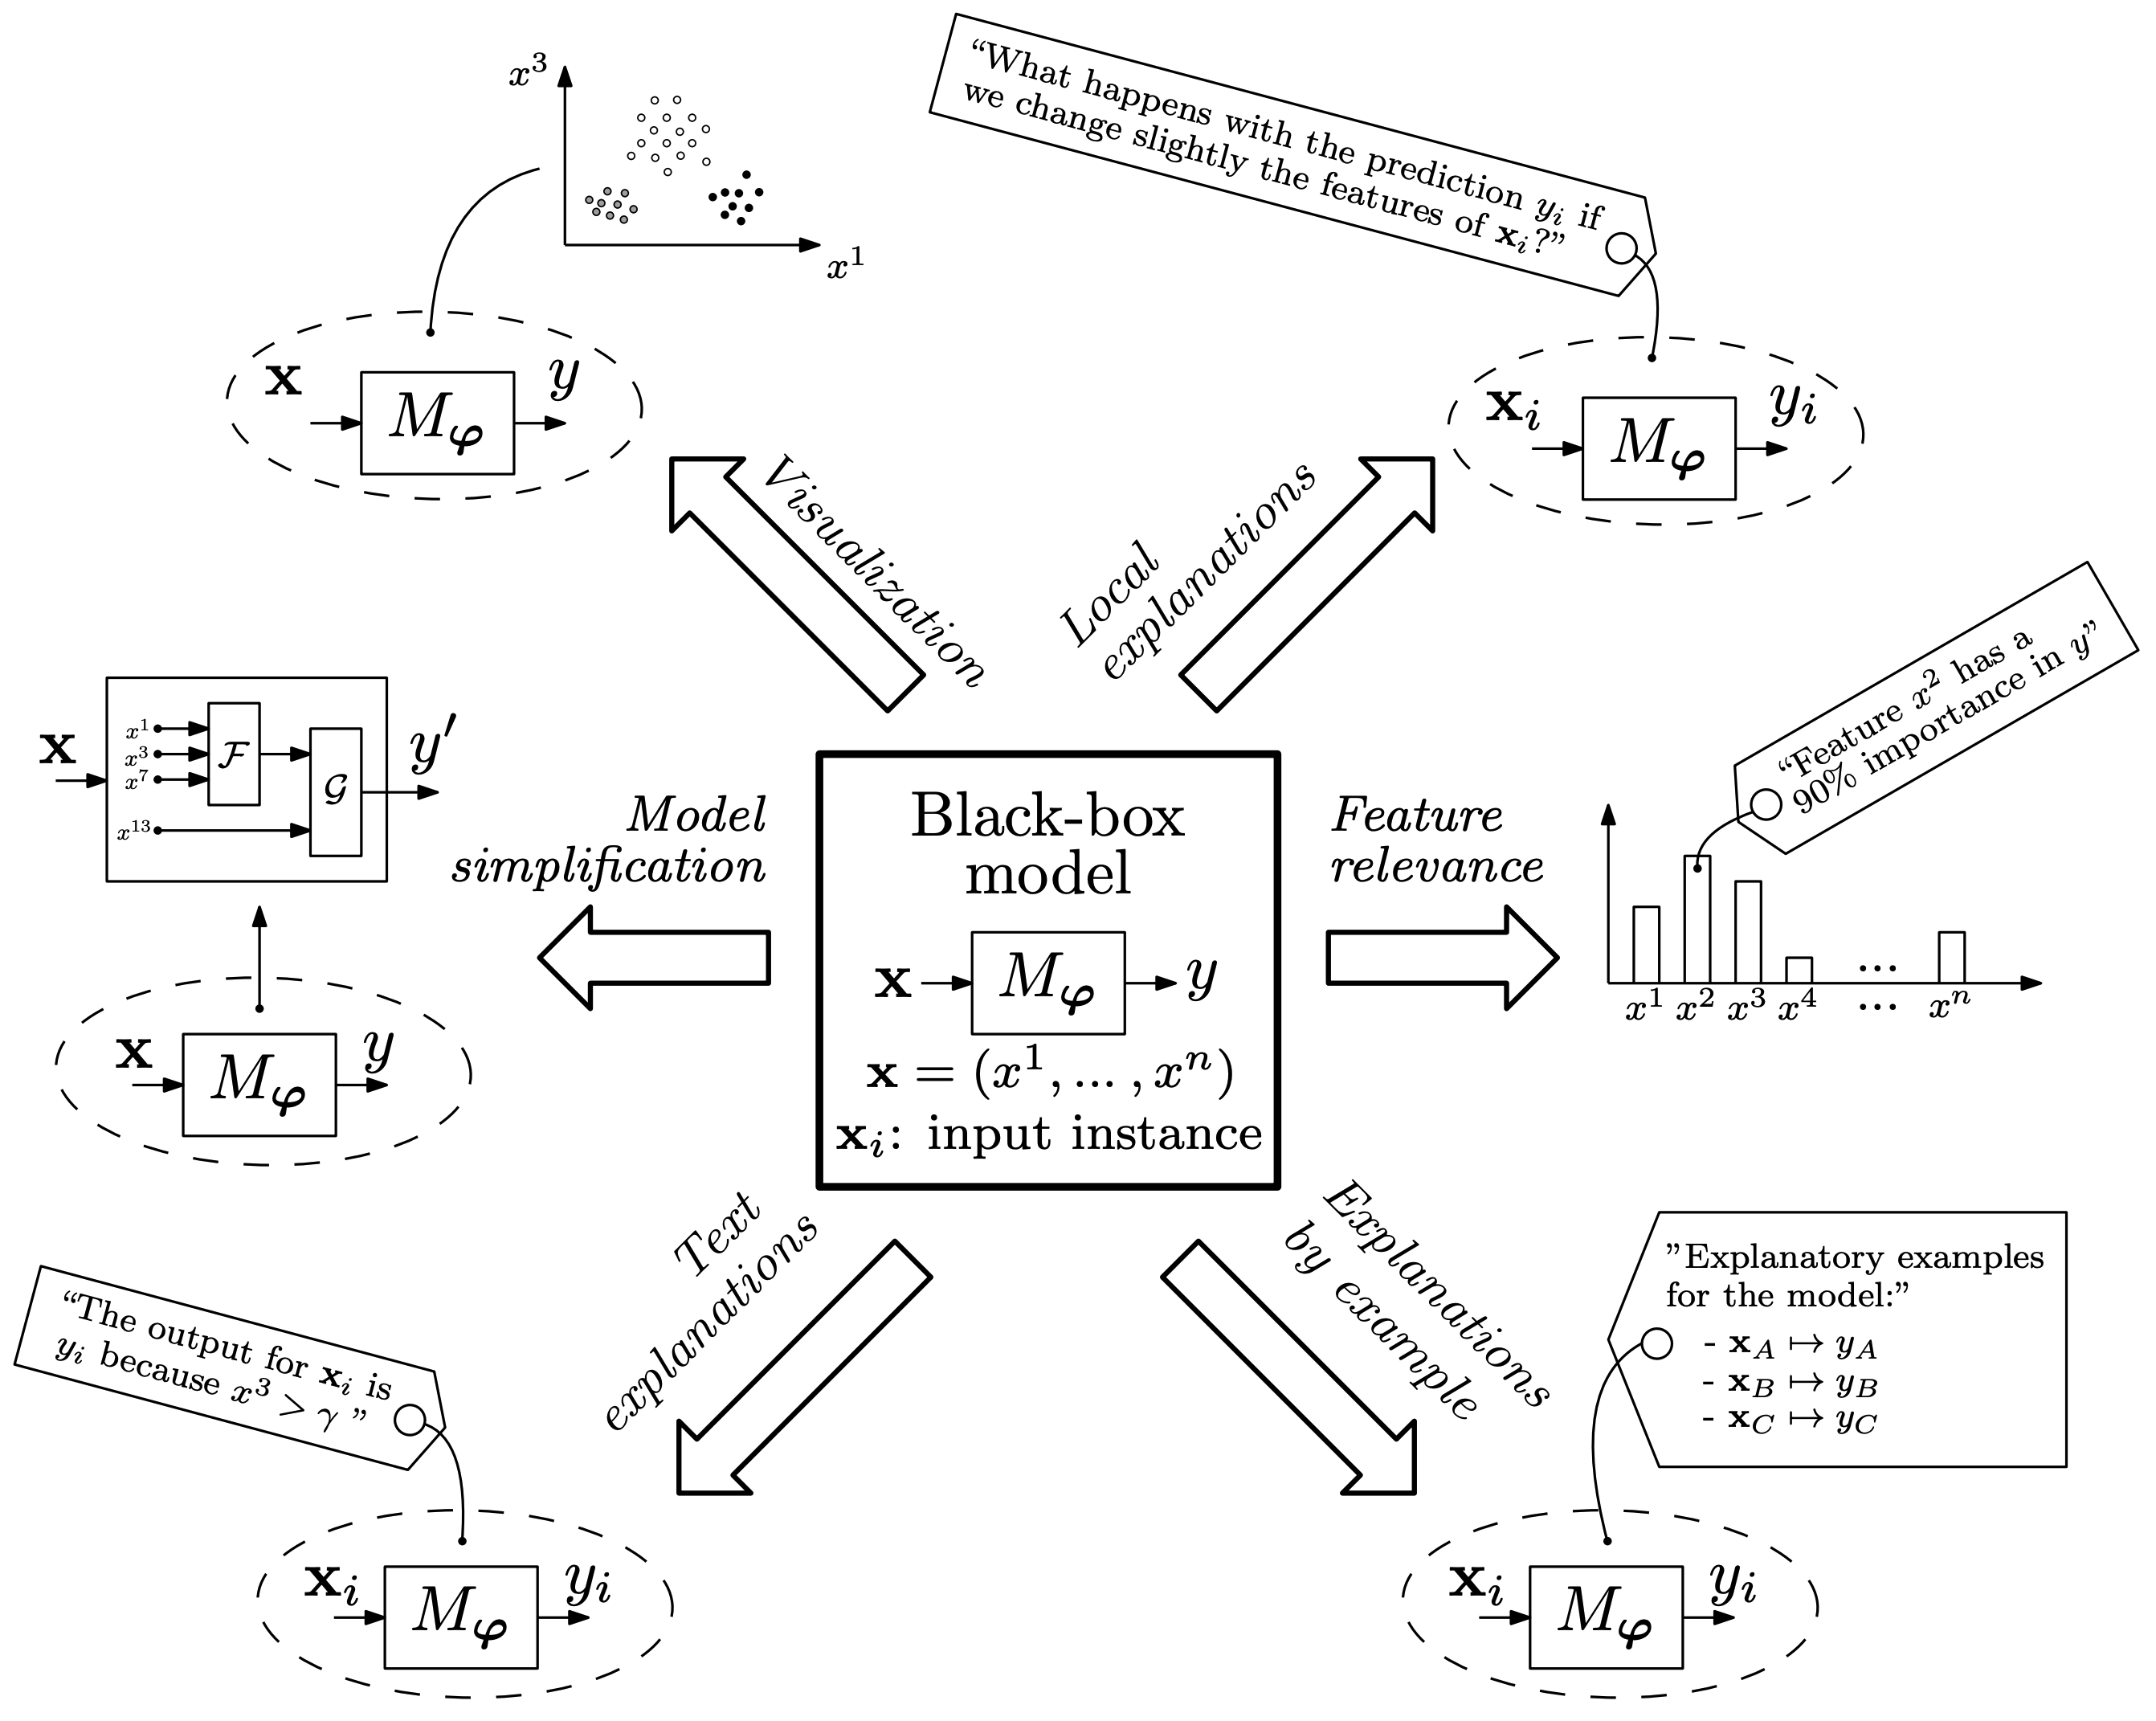
\includegraphics[scale=0.177]{visual_representation_explanation_types.png}
  \end{center}
  \begin{flushright}
    {\vspace{-16pt} \tiny Source:~\citet{Arrieta:2020}}
  \end{flushright}
\end{frame}

\begin{frame}{Explanations by Example}{}
  \begin{columns}
    \begin{column}{0.45\textwidth}
      \begin{itemize}
        \setlength{\itemsep}{22pt}
        \item Common approach in human learning via \green{prototypical examples}
        \item \blue{\textbf{Example}}: \href{https://quickdraw.withgoogle.com/}{Google Quick, Draw!}~\citep{Cai:2019}
          \begin{itemize}
          \setlength{\itemsep}{8pt}
            \item Like charades or the old TV~show ``\href{https://en.wikipedia.org/wiki/Win,_Lose_or_Draw}{Win, Lose, or Draw}''
            \item Given a prompt and the user draws it
            \item AI tries to guess the picture
          \end{itemize}
      \end{itemize}
    \end{column}
    \begin{column}{0.1\textwidth}
    \end{column}
    \begin{column}{0.45\textwidth}
      \onslide<2->{%
        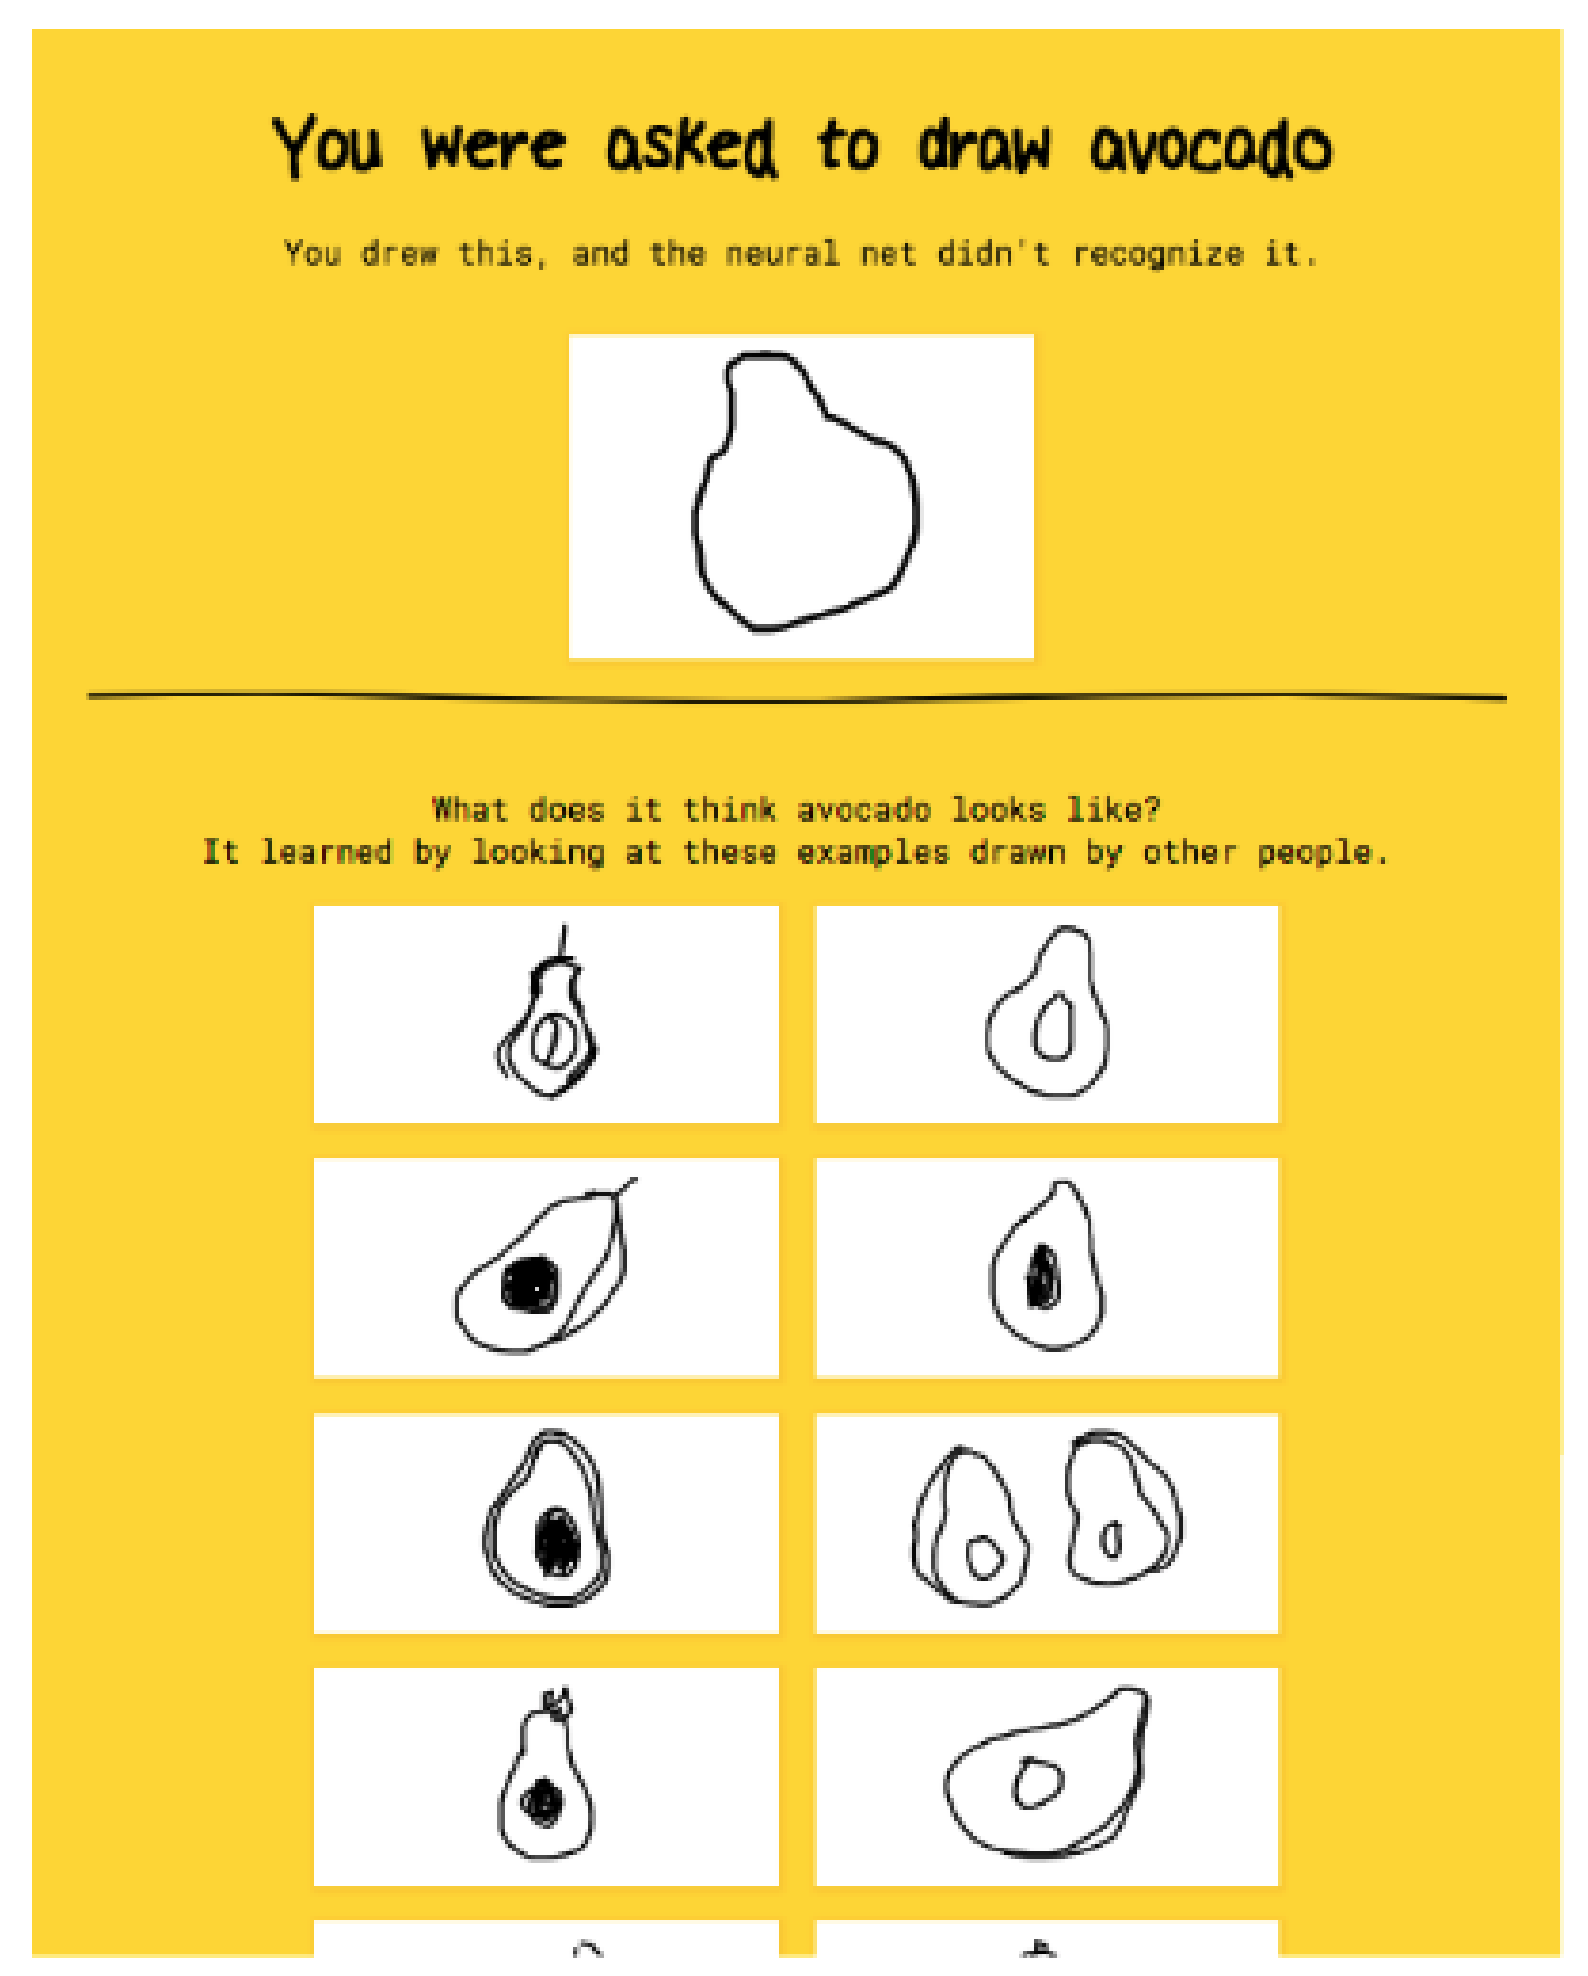
\includegraphics[scale=0.20]{avocado_quick_draw.png}
      }
    \end{column}
  \end{columns}
\end{frame}

\begin{frame}{Local Explanation}
  \blue{\textbf{Obvious Question}}: Why was this \textit{particular instance} mispredicted?

  \vspace{16pt}
  \begin{center}
    \onslide<2->{
          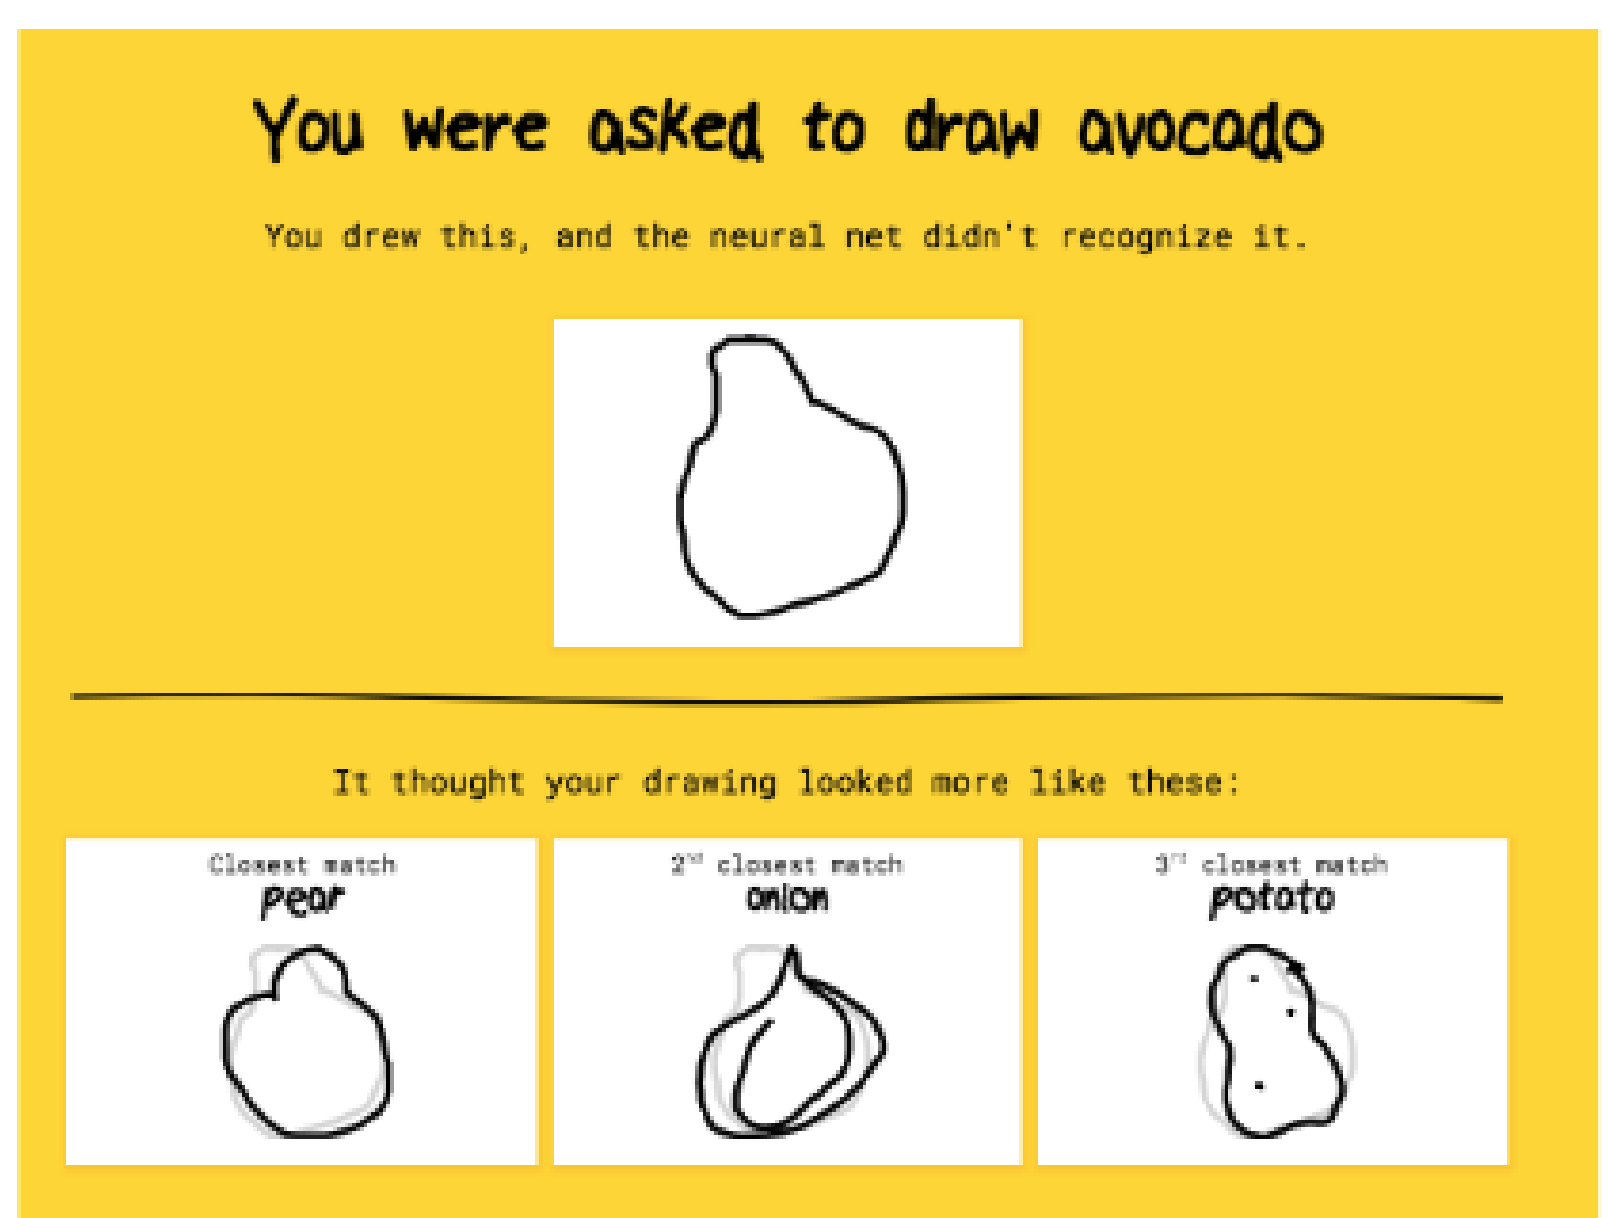
\includegraphics[scale=0.264]{avocado_alternates_quick_draw.png}
    }
  \end{center}
\end{frame}

\section{Explainability Approaches}

\transitionFrame{\LARGE Post-Hoc Explainability Approaches: \\\vspace{6pt} Two Categories}

\subsection{Random-Forest Specific}
\begin{frame}{Random Forest Explainability Approaches}
  \noindent
  Random forests~(RF) are among the best performing ML algorithms for a wide variety of domains.

  \vspace{18pt}
  \noindent
  First we examine, post-hoc RF explainability algorithms
  \begin{itemize}
    \item \green{\textbf{Post-Hoc}}: Refers to the application of explainability methods \textit{after} model training~\citep{Molnar:2019}
  \end{itemize}
\end{frame}

\begin{frame}{Explainability by Simplification: Rule Extraction}
  A decision tree can be viewed as a set of ordered rules
  \begin{itemize}
    \item RF simplification methods seek to extract a compact set of \textit{simple} rules from these complex models.
  \end{itemize}

  \vspace{16pt}
  \noindent
  \green{\textbf{Various Ideas}}:
  \begin{itemize}
    \setlength{\itemsep}{10pt}
    \item Convert an RF into a single decision tree
    \item Focus on extract \textit{more representative rules} by focusing on those that are most prominent
    \item Use local search (e.g.,~hill climbing) to construct a set of rules approximating the RF
  \end{itemize}
\end{frame}

\begin{frame}{Feature Relevance}
  \green{\textbf{Extensive Previous Work}} -- Topics include:
  \begin{itemize}
    \setlength{\itemsep}{15pt}
    \item Assess importance of individual features by computing how much the model's accuracy drops after excluding the feature
    \item Estimate the importance of a feature by measuring how much it needs to change to affect the model's prediction.  \textit{Intuition}: Small change, high importance
    \item Determine which subsets of features interact together
  \end{itemize}
\end{frame}

\subsection{Model Agnostic}

\begin{frame}{Model Agnostic Explainability Approaches}
  \textbf{\blue{Primary Advantage}}: Generally applicable and flexible

  \vspace{18pt}
  \textbf{\blue{Primary Disadvantage}}: Cannot utilize a model's distinct to produce better explanations
  \begin{itemize}
    \item Slower
    \item Lower fidelity
    \item Provides limited to no insight into the operation of the learning algorithm itself
  \end{itemize}
\end{frame}

\begin{frame}{Explainability by Simplification: LIME}
  \noindent
  \textbf{Greatest Hit}: \underline{L}ocal \underline{I}interpretable \underline{M}odel-Agnostic \underline{E}xplanations~\citep{Ribeiro:2016}
  \begin{itemize}
    \item Approximates an opaque model locally via a transparent model (e.g.,~linear model or decision tree)
  \end{itemize}

  \vspace{18pt}
  \noindent
  \textbf{Thought Experiment}: Create a model trying to identify the type of animal in a picture
  \begin{itemize}
    \item Necessitates high level features
    \item LIME transforms input data into \textit{interpretable representations} understandable by humans
  \end{itemize}
\end{frame}

\begin{frame}{Counterfactuals}
  \begin{itemize}
    \setlength{\itemsep}{18pt}
    \item Instance as close as possible to an instance of interest but for which the model classifies the alternate instance differently

    \item \textit{\green{Example}}: Application is denied a loan.  A counterfactual could say which factors, if changed, would have led to the loan application being improved.
  \end{itemize}
\end{frame}

\begin{frame}{Feature Relevance: SHAP}
  \noindent
  \textbf{Greatest Hit}: \underline{Sh}apley \underline{A}dditive ex\underline{P}lanations~\citep{Lundberg:2017}
  \begin{itemize}
    \item \textbf{\green{Shapley Value} of a Feature}: Average, expected marginal contribution to the model's decision
    \item Strong mathematical foundation in conditional game theory
  \end{itemize}

  \vspace{18pt}
  \noindent
  \textbf{Basic Objective}: Train a linear model around the instance to be explained
  \begin{itemize}
    \item Linear models make the weight of each feature obvious
  \end{itemize}

  \vspace{18pt}
  \noindent
  \textbf{Strong Assumption}: Each feature is independent
\end{frame}

\begin{frame}{Visual Explanation: ICE}
  % \begin{columns}
  %   \begin{column}{0.5\textwidth}
      \textbf{Greatest Hit}: \underline{I}ndividual \underline{C}onditional \underline{E}xpectation~\citep{Goldstein:2015}

      \begin{itemize}
        \setlength{\itemsep}{10pt}
        \item Operates on the instance level
        \item Depicts model decision boundary as a function of a single feature
      \end{itemize}

      \vspace{8pt}
      \begin{center}
        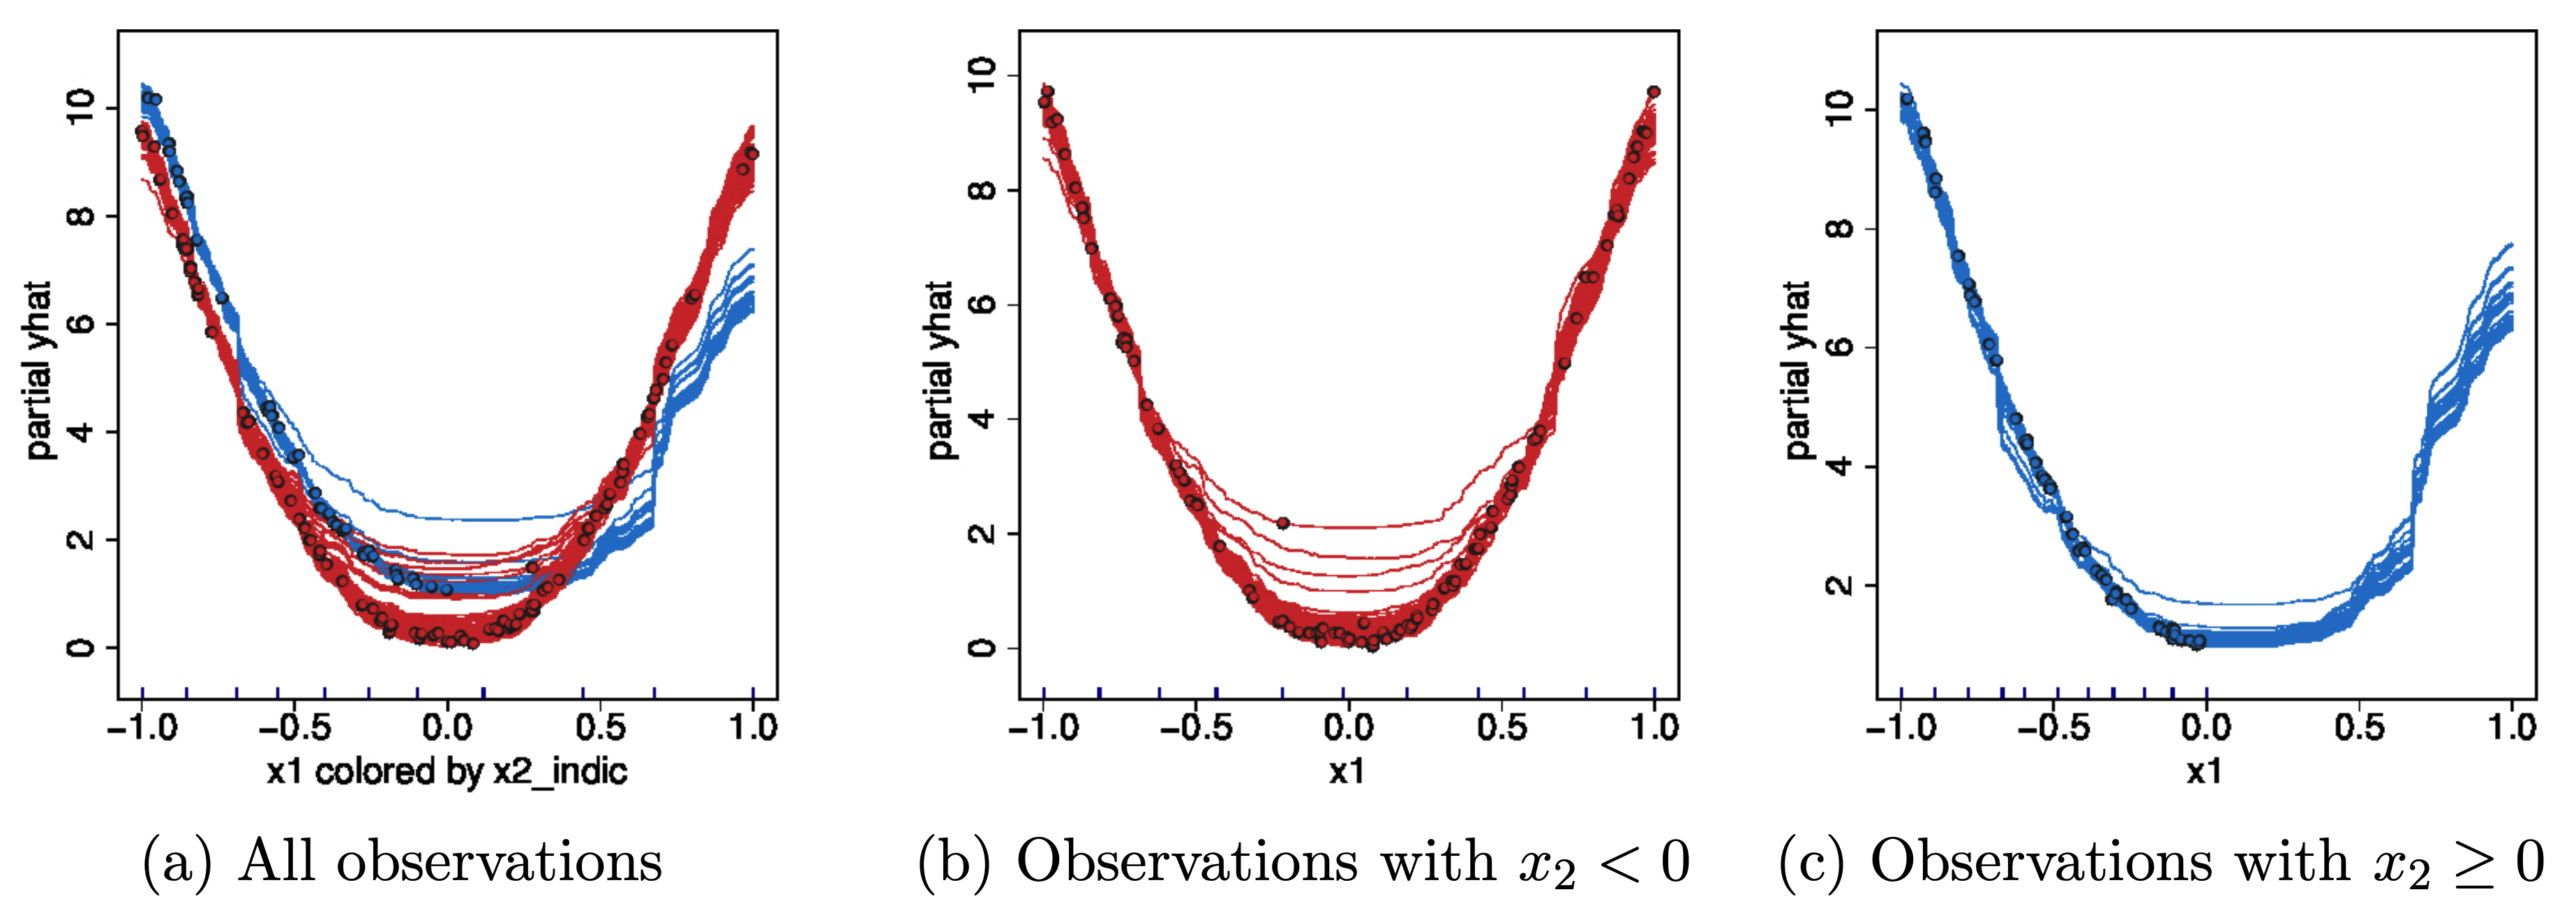
\includegraphics[scale=0.2]{ice_plots.png}
      \end{center}
    % \end{column}
  % \end{columns}
\end{frame}

\section{Conclusions}
\begin{frame}{Closing Thoughts}{}
  \textbf{Audience First}: The best visualization depends on the needs/requirements of the particular audience targeted.

  \vspace{18pt}
  \textbf{Try Diverse Methods}: Relying one algorithm/explanation type only gives a partial picture

  \vspace{18pt}
  Like all machine learning systems, XAI is vulnerable to adversarial attacks.
\end{frame}
\begin{frame}{Good (Ordered) Rules of Thumb}{}
  \begin{enumerate}
    \setlength{\itemsep}{16pt}
    \item If explainability is essential for the application, try a transparent model first.
    \item If a transparent model does not perform well enough and \textit{you lose the explainability benefit}, use an opaque model.
    \item Employ a \textit{feature-relevance method} to get an instance-specific estimate of feature influence.
    \item Use a \textit{model simplification approach} to see if the locally important features are globally influential.
    \item Use a visualization technique to plot the decision boundary as a function of important features
  \end{enumerate}
\end{frame}

\begin{frame}{Table of Contents}[noframenumbering]
  \tableofcontents
\end{frame}

\appendix

\begin{frame}[allowframebreaks]{Bibliography}{}
  {\tiny
    \frametitle{References}
    \bibliography{bib/ref.bib}
    \bibliographystyle{unsrtnat}
  }
\end{frame}
\end{document}
